\subsection{Glyph: \glyph{Logic arc}}
\label{sec:logicArc}

\glyph{Logic arc} is used to represent the fact that an entity \add{pool or a logical operator} influences
the outcome of a logic operator.

\begin{glyphDescription}

\glyphSboTerm
SBO:0000398 ! logical relationship

\glyphOrigin
\corr{Any}{One} \glyph{EPN} (\sect{EPNs}) or \glyph{logical operator} (\sect{logic}).

\glyphTarget
\corr{Any}{One} \glyph{logical operator} (\sect{logic}) \add{or \glyph{EPN} (\sect{EPNs})}.

\glyphSymbol
No particular symbol is used to represent a \glyph{logic arc}, as shown in \fig{logicArc}.

\end{glyphDescription}

\begin{figure}[H]
  \centering
  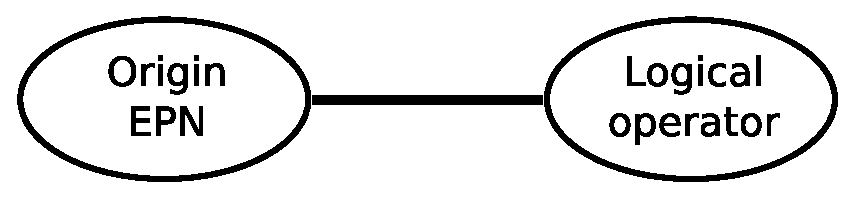
\includegraphics{images/logicArc}
  \caption{The \PD glyph for \glyph{logic arc}.}
  \label{fig:logicArc}
\end{figure}
